% Finished August 17, 2012
% Split in half October 15, 2013.
% Put into VUW thesis format (with Figure numbers) November 2013.

\documentclass[12pt, a4paper, twoside, openright]{book}

\usepackage{vuwthesis} % sets up some local things, mostly the front page

\setlength{\intextsep}{12pt} % set space above and below in-line float
\setlength{\abovecaptionskip}{0pt} % set space between figure and caption.

\usepackage{amssymb, amsmath}
\usepackage{tikz}

\newcommand{\beff}{\ensuremath{b_{\mathrm{eff}}}}
\newcommand{\ewf}{\ensuremath{\epsilon_{\mathrm{wf}}}}

\usepackage{etoolbox}
\newtoggle{compilealone}
\toggletrue{compilealone}

\author{Nat Lund}
\title{Chapter 1: Introduction}

\begin{document}
\chapter{Introduction}\label{C:intro}

\section{Background}

How fast is the water at the bottom of the canal? Is it moving or at rest? The first person to provide an answer to this question (indeed, perhaps the first to ask it; entertainment was limited in those days) was probably Daniel Bernoulli. He claimed: the water is at rest. This pronouncement was made in 1738, but it was not until the twentieth century that this notion came to be accepted as universally valid. This notion is of course the `no slip' boundary condition of fluid mechanics.

The foundations of fluid mechanics were laid by Navier and Stokes by about 1840. Their eponymous equation captured the fact that an element of fluid obeys Newton's Second Law $F=ma$ just as surely as `solid' matter. But the Navier-Stokes equations are not enough: While they describe behaviour in the \emph{bulk} of the fluid, to generate a complete description of the fluid, we need information about what goes on at the \emph{boundaries.}

Unlike the case of the bulk fluid obeying Newton's universal laws of motion, there seemed to be no fundamental \emph{a priori} principle at work on the boundary. However, there was a body of experimental work. Interestingly, no clear picture --- let alone a clear principle --- had emerged from the experiments.  Bernoulli's early result had later been contradicted by experiments showing \emph{slip.} That is, the fluid in contact with the solid surface moved, or slipped, along the solid. By the 1840s, the issue had become sufficiently controversial that Stokes himself was commissioned to sort the matter out. At length, he determined that fluid did \emph{not} slip along the solid surface. But the matter didn't end there; for example, Helmholtz found evidence of slip in the 1860s. The issue wasn't fully settled until 1927, when Tausz and K\"orosy published a book in which previous evidence of slip was dismissed as experimental artefact. An overview of this early history (and much more) is available in the excellent 2005 review article by Chiara Neto \emph{et al} \cite{NetoReview2005}.

Thus, by the early twentieth century, the no slip boundary condition had become cemented in fluid mechanics textbooks. However, by the the twenty-first century, evidence was beginning to accumulate that the no slip condition sometimes does not hold.
Before discussing this, it will help to introduce some mathematical machinery --- specifically, the concept of \emph{slip length.}

\section{Slip Length}

Let us consider what is surely the simplest case of fluid flow: Couette flow.  In this canonical regime, some fluid sits between two parallel solid plates. One of the plates is moving at a constant velocity, with respect to the other plate. (For clarity we shall often assume that the bottom plate is stationary, and the top plate moves; another convention is that the two plates have equal and opposite velocities.) The plates are considered to be infinite planes; likewise, the interstitial fluid extends infinitely in all horizontal directions, so that there are no `edges' to the system. We are interested in the flow velocity field of the fluid in the steady state.  A schematic diagram of a Couette flow system is in Figure (\ref{Couettesystem}).
\clearpage

\begin{figure}[ht]
\centering
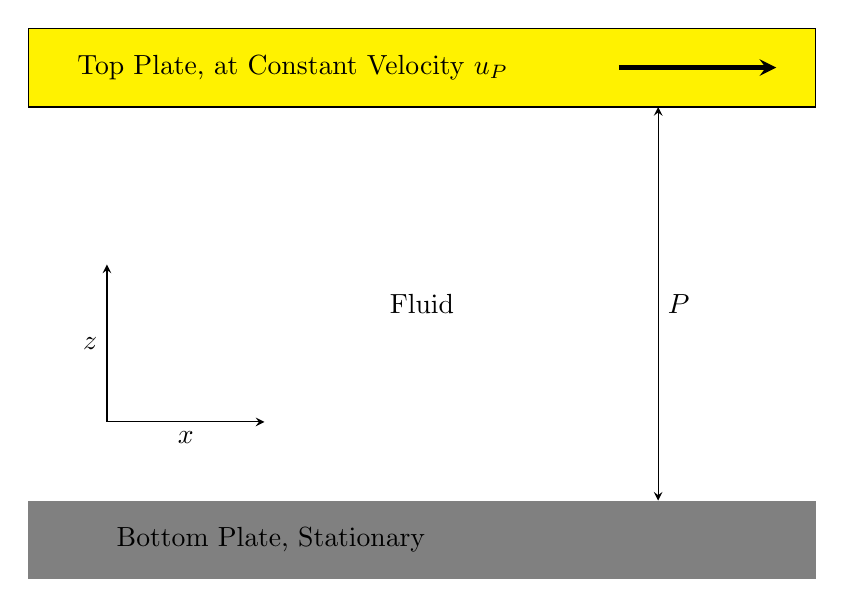
\begin{tikzpicture}    [> = stealth]

\filldraw[fill=yellow, draw=black] (0,5) rectangle (10,6);
\fill[color=gray] (0,0) rectangle (10,-1);

\node at (0.5,5.5) [right] {Top Plate, at Constant Velocity $u_{P}$};
\node at (5,2.5) {Fluid};
\node at (1,-0.5) [right] {Bottom Plate, Stationary};

\draw [->, ultra thick] (7.5,5.5) -- +(2,0);

\draw [<->] (1,3) -- node[left] {$z$} ++(0,-2) -- node[below] {$x$} +(2,0);

\draw [<->] (8,0) -- node[right] {$P$} +(0,5); 

\end{tikzpicture}
\caption{The system of Couette flow} \label{Couettesystem}
\end{figure}

This setup is amenable to experimental measurement; the point of theoretical physics is to generate a prediction of the measurements using mathematical reasoning.  To that end, we need a mathematical model of the physical situation.
We work in $\mathbb{R}^{3}$, with $z$ being the vertical direction, and $x$ the left-to-right horizontal direction. The fluid is modeled as a \emph{continuum} velocity field $\vec{u}(x,y,z) = (u,v,w) $ obeying the Navier-Stokes equations at all points. The boundaries of the fluid -- the two plates -- are modeled as perfect $x,y$ planes, separated by a width $P$. The bottom boundary is the plane $z=0$, the top the plane $z=P$.
The bottom boundary is stationary, while the top boundary has a constant velocity $\vec{u}_P$ in the $x$ direction (with magnitude $u_{P}$). 

To solve the Navier-Stokes equations, a boundary condition is required. Let's start with the simple classical case of no slip. Since the fluid sticks to the boundaries, the fluid at the bottom boundary has zero velocity, while fluid at the top boundary has velocity $\vec{u}_{P}$. 
The fluid has \emph{viscosity}, that is, a layer of fluid atoms sliding over another layer causes a shear stress that tends to accelerate the lower layer.  By this mechanism, the driving plate drives the entire bulk fluid, as the driving velocity propagates down through the fluid.
%The fluid is driven by the driving plate, and viscosity causes shear stress, accelerating %fluid in the bulk. 
The steady-state solution is that the fluid velocity is in the $x$ direction only, with a magnitude $u(z)$ that changes linearly between 0 at the bottom and $u_{P}$ at the top:

\begin{equation}
u(z) = \frac{z}{P}u_{P}  
\end{equation}

A schematic of Couette flow with its characteristic linear velocity gradient appears in Figure (\ref{Couetteflow}).

\begin{figure}[ht]
\centering
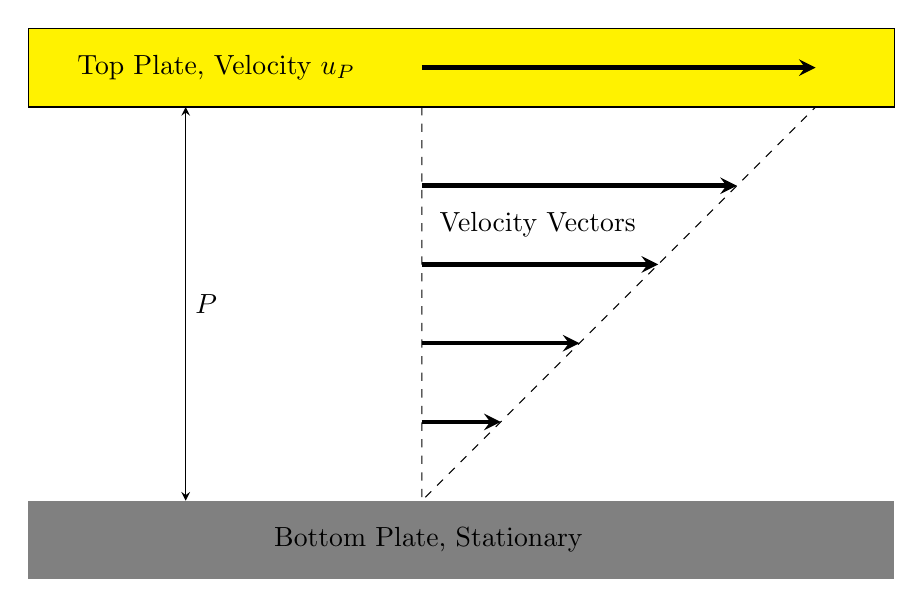
\begin{tikzpicture}    [> = stealth]

\filldraw[fill=yellow, draw=black] (-1,5) rectangle ++(11,1);
\fill[color=gray] (-1,0) rectangle (10,-1);

\node at (-0.5,5.5) [right] {Top Plate, Velocity $u_{P}$};
\node at (4.1,3.5) [right] {Velocity Vectors};
\node at (2,-0.5) [right] {Bottom Plate, Stationary};

\draw [->, ultra thick] (4,5.5) -- +(5,0);

\draw [<->] (1,0) -- node[right] {$P$} +(0,5); 

% x,z axes
%\draw [<->] (1,3) -- node[left] {$z$} ++(0,-2) -- node[below] {$x$} +(2,0); 

\foreach \z in {1,2,3,4}
  \draw [->, ultra thick] (4,\z) -- +(\z,0);

\draw [dashed] (4,5) -- +(0,-5) -- +(5,0);  

\end{tikzpicture}
\caption{Couette flow} \label{Couetteflow}
\end{figure}

Now let's relax the no slip condition and consider some kind of \emph{slip} boundary condition. The simplest such condition is that there is a finite slip velocity at the surface, and that velocity is proportional to the \emph{shear rate} in the fluid. This condition was first proposed by Navier:

\begin{equation}
u_{\mathrm{slip}} = b \frac{\partial u}{\partial z}
\end{equation}

The constant of proportionality $b$, has units of length, and accordingly is known as the \emph{slip length.}

Since the shear stress is proportional to the shear rate, the Navier slip relation says that the shear stress on the fluid at the boundary is proportional to the fluid velocity at the boundary.

In the model in use here, the slip length has a simple geometric interpretation: 
The velocity gradient at the wall may be linearly extrapolated \emph{into} the wall. The distance into the wall at which the velocity \emph{would} be zero, is the slip length.

Couette flow with a non-zero slip length is shown in Figure (\ref{Couetteslip}).

\begin{figure}[ht]
\centering
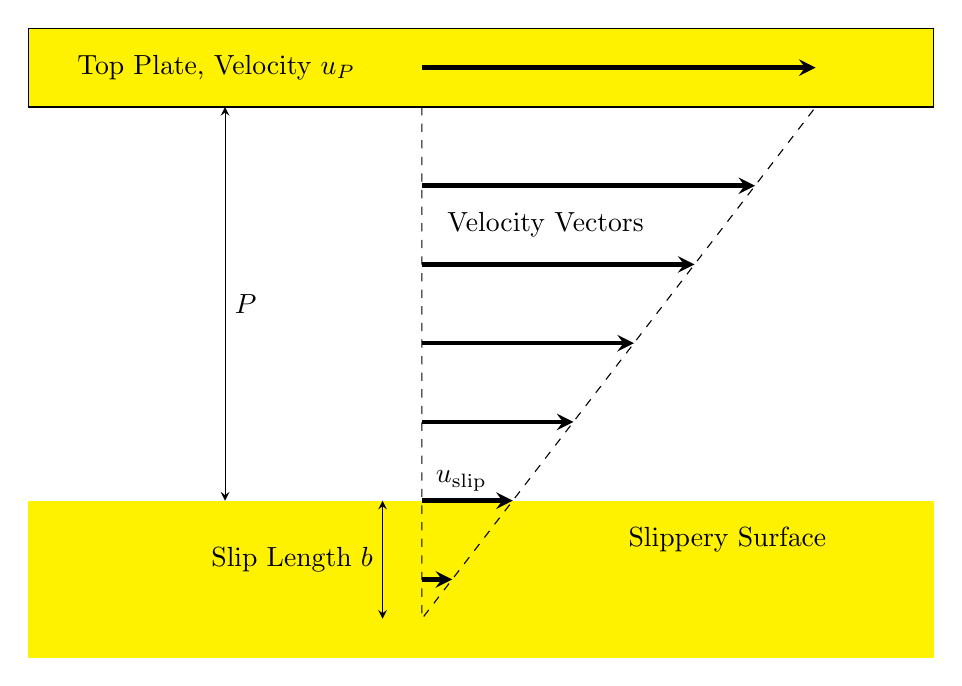
\begin{tikzpicture}    [> = stealth]

\filldraw[fill=yellow, draw=black] (-1.5,5) rectangle ++(11.5,1);
\fill[color=yellow] (-1.5,0) rectangle ++(11.5,-2);

\node at (-1,5.5) [right] {Top Plate, Velocity $u_{P}$};
\node at (3.7,3.5) [right] {Velocity Vectors};
\node at (6,-0.5) [right] {Slippery Surface};

\draw [->, ultra thick] (3.5,5.5) -- +(5,0);

\draw [<->] (1,0) -- node[right] {$P$} +(0,5); 

% x,z axes
%\draw [<->] (1,3) -- node[left] {$z$} ++(0,-2) -- node[below] {$x$} +(2,0); 

\foreach \z in {-1,0,1,2,3,4}
  \draw [->, ultra thick] (3.5,\z) -- +(\z*0.76923 + 1.1545 ,0);

\draw [dashed] (3.5,5) -- +(0,-6.5) -- +(5,0); 

\draw [<->] (3,0) -- node[left] {Slip Length $b$} +(0,-1.5); 

\node at (4,0)[above] {$u_{\mathrm{slip}}$};

\end{tikzpicture}
\caption{Couette flow with slip} \label{Couetteslip}
\end{figure}

At this point we stop to emphasize that the slip length is a feature of the \emph{mathematical model.} We have assumed two things: First, the boundary between fluid and solid is a perfect Euclidean plane. Second, the fluid is a continuum, allowing for a well-defined velocity gradient at the boundary. Reconciling this Platonic ideal with a real physical experiment is non-trivial. We shall go into some depth with this issue shortly.

The slip length is a property of the fluid/solid interface, and can in principle vary in space. This leads us to the concept of \emph{effective slip length}, the calculation of which is the subject of this thesis.

%\clearpage
\section{Effective Slip Length}

Working again with the same model, let us assume the slip length $b$ is a parameter that varies over the solid surface. 
This could model the case when the surface \emph{material} changes spatially, eg.\ high-slip Teflon regions on a no-slip metal surface.
Again, we seek a velocity flow field description of the fluid. In this case, a simple solution is not readily apparent --- the problem has essentially gained an extra dimension. In fact, there are no known analytical solutions to this general problem.

The flow field near the surface will no longer be a straightforward laminar flow, but will be perturbed by the spatial variations in slip length. However, we would expect those perturbations to decay with increasing height above the surface. At sufficient height, the perturbations will be essentially zero, and the flow will be uniform laminar flow. This uniform flow has a shear rate that does not vary over space.  Therefore, the velocity gradient can be extrapolated down to the solid surface, and \emph{into} the surface, defining an \emph{effective} slip length.

This is illustrated in Figure (\ref{effslip}).

\begin{figure}[ht!]
\centering
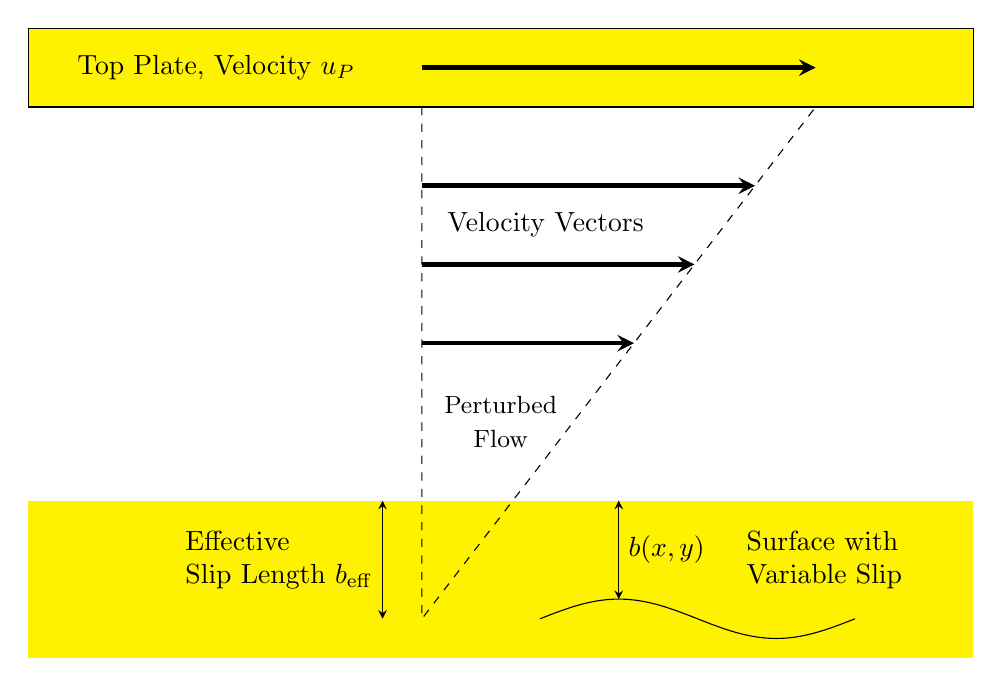
\begin{tikzpicture}    [> = stealth]
\renewcommand{\baselinestretch}{1.00}

\filldraw[fill=yellow, draw=black] (-1.5,5) rectangle ++(12,1);
\node at (-1,5.5) [right] {Top Plate, Velocity $u_{P}$};
\draw [->, ultra thick] (3.5,5.5) -- +(5,0);
 
\fill[color=yellow] (-1.5,0) rectangle ++(12,-2); 
 
\foreach \z in {2,3,4}
  \draw [->, ultra thick] (3.5,\z) -- +(\z*0.76923 + 1.1545 ,0);
\draw [dashed] (3.5,5) -- +(0,-6.5) -- +(5,0); 
\node at (3.7,3.5) [right] {Velocity Vectors};

\node at (4.5,1) [align=center] {\small Perturbed\\ \small Flow};

\node at (7.5,-0.75) [right,align=left] {Surface with\\ Variable Slip};

\draw [<->] (3,0) -- node[left, align=left] {Effective\\Slip Length $b_{\mathrm{eff}}$} +(0,-1.5); 

\draw (5,-1.5) sin ++(1,0.25) cos ++ (1,-0.25) sin ++(1,-0.25) cos ++(1,0.25);
\draw[<->] (6,0) -- node[right] {$b(x,y)$} ++(0,-1.25);

\end{tikzpicture}
\caption{Effective slip length} \label{effslip} 
\end{figure}


\vspace{1em}
The far-field flow of the system is equal to that of an \emph{effective} system, defined as follows:  The effective system has the same top boundary condition, but has a no-slip boundary condition holding on a lower surface located distance $\beff$ below the surface of the original system.

The no-slip plane of the effective system is denoted the \textbf{effective no-slip plane.}
Hence, the effective slip length of the system of perturbed Couette flow is the distance that the effective no-slip plane lies below the physical surface plane.  See Figure (\ref{effnoslip}).


\begin{figure}[ht!]
\centering
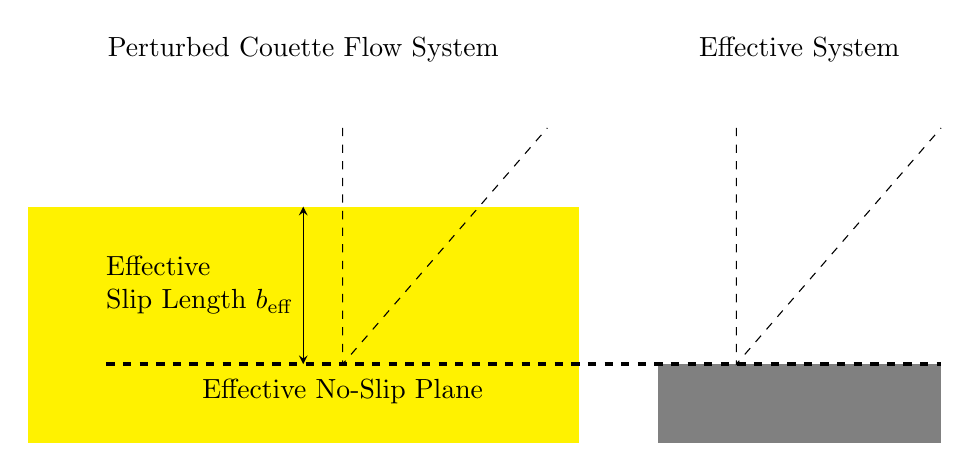
\begin{tikzpicture}  [> = stealth]
\renewcommand{\baselinestretch}{1.00}

\fill[color=yellow] (0,0) rectangle (7,-3);

\draw [<->] (3.5,0) -- node[left, align=left] {Effective\\Slip Length $b_{\mathrm{eff}}$} ++(0,-2);
\draw[dashed] (4,1) -- ++(0,-3) -- ++(2.6,3);

\fill[color=gray] (8,-2) rectangle ++(3.6,-1);
\draw[dashed] (9,1) -- ++(0,-3) -- ++(2.6,3);

\draw[very thick, dashed] (1,-2) -- ++(10.6,0);
\node at (4,-2.35) {Effective No-Slip Plane};

\node at (3.5,2) {Perturbed Couette Flow System};
\node at (9.8,2) {Effective System};
\end{tikzpicture}
\caption{Effective no-slip plane} \label{effnoslip} 
\end{figure}


\clearpage

\section{Effective Slip Length of Rough Surface}

We now extend the model, allowing the solid surface to be \emph{rough} rather than just flat. 
%The surface is now \emph{rough}, perhaps corrugated. 
We allow the local slip length to vary over the surface, as before.

%The definition of effective slip is the same as before, but with an important extension: The position of the solid/liquid interface is now a \emph{range.} Therefore, the effective slip length can be defined with respect to any position in that range. We let the surface be a function $h(x,y)$, (nominally centered at $z=0$), bounded by $h_{\mathrm{min}}$ and $h_{\mathrm{max}}$. Define $\Delta h = h_{\mathrm{max}} - h_{\mathrm{min}}$. Then plausible definitions of $\beff$ lie in the range $[b_{0}, b_{0} + \Delta h]$, where $b_{0}$ is the minimum \emph{effective} slip length --- not the minimum \emph{local} slip length.

The definition of effective slip now acquires a subtlety: the solid-liquid interface is no longer a flat plane.  The system still behaves like an effective system with an effective no-slip plane located below the physical surface.  But now the distance from the physical surface to the effective no-slip plane is ambiguous. In principle, one could measure the distance from the troughs of the rough surface, or the peaks, or any point in between. 
See Figure (\ref{effsliprough}). In fact, as we shall see in Chapter 3, this ambiguity caused apparent contradictions in the measurement of effective slip on rough surfaces, as different researchers adopted different conventions.



\begin{figure}[ht]
\centering
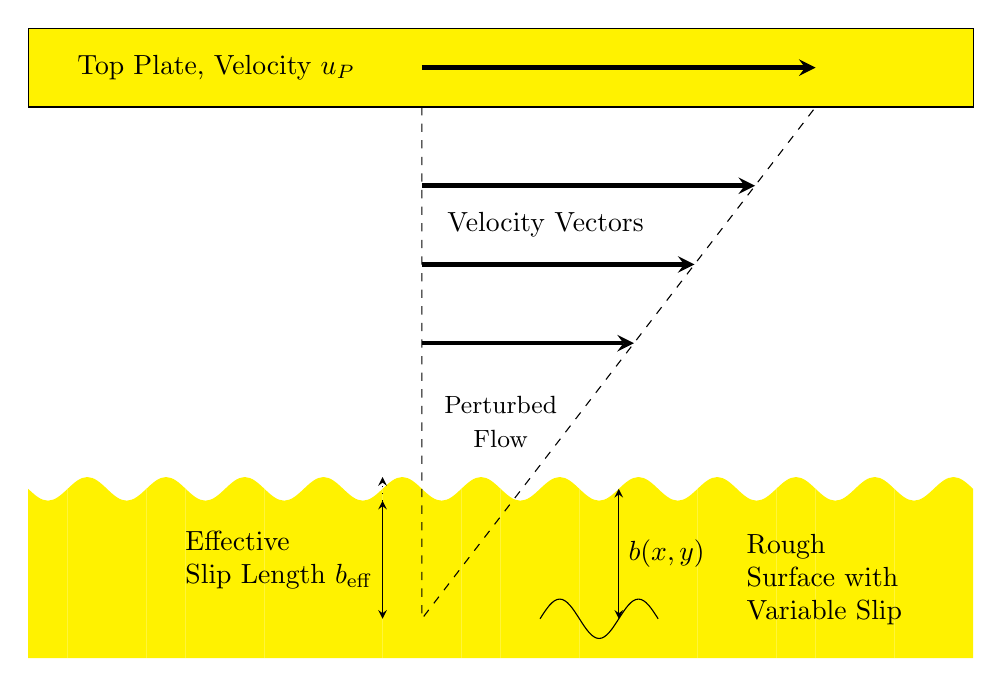
\begin{tikzpicture}    [> = stealth]
\renewcommand{\baselinestretch}{1.00}

\filldraw[fill=yellow, draw=black] (-1.5,5) rectangle ++(12,1);
\node at (-1,5.5) [right] {Top Plate, Velocity $u_{P}$};
\draw [->, ultra thick] (3.5,5.5) -- +(5,0);

%\fill[color=yellow] (-1.5,0) rectangle ++(12,-2);
\foreach \x in {-1,...,10}
               {   \fill[color=yellow] (\x,-2) -- ++(0,2.15) sin ++(0.25,0.15)
                   cos ++(0.25,-0.15) |- ++(-0.5,-2.15);   }
\foreach \x in{-2,...,9} 
              {   \fill[color=yellow] (\x+ 0.5,-2) -- ++(0,2.15) sin ++(0.25,-0.15)
                  cos ++(0.25,0.15) |- ++(-0.5,-2.15);    }

\foreach \z in {2,3,4}
  \draw [->, ultra thick] (3.5,\z) -- +(\z*0.76923 + 1.1545 ,0);
\draw [dashed] (3.5,5) -- +(0,-6.5) -- +(5,0); 
\node at (3.7,3.5) [right] {Velocity Vectors};

\node at (4.5,1) [align=center] {\small Perturbed\\ \small Flow};

\node at (7.5,-1) [right,align=left] {Rough\\Surface with\\ Variable Slip};

\draw [<->] (3,0) -- node[left, align=left] {Effective\\Slip Length $b_{\mathrm{eff}}$} +(0,-1.5); 
\draw [dotted, ->] (3,0) -- +(0,0.3);

\draw (5,-1.5) sin ++(0.25,0.25) cos ++(0.25,-0.25) sin ++(0.25,-0.25)
               cos ++(0.25,0.25) sin ++(0.25,0.25) cos ++(0.25,-0.25);
\draw[<->] (6,0.15) -- node[right] {$b(x,y)$} ++(0,-1.65);

\end{tikzpicture}
\caption{Effective slip length of rough surface} \label{effsliprough} 
\end{figure}

\clearpage

Defining a nominal surface plane at the \textbf{tops of the peaks} of the surface roughness is a defensible choice.  See Figure (\ref{rougheffnoslip}). That way, pure bulk conditions hold above the nominal surface.
Furthermore, physical instruments probing the position of the surface would tend to encounter the tops of the peaks, and record this as the surface position.
Incidentally, this convention has the effect of maximizing effective slip lengths measured on rough surfaces.  


\begin{figure}[ht!]
\centering
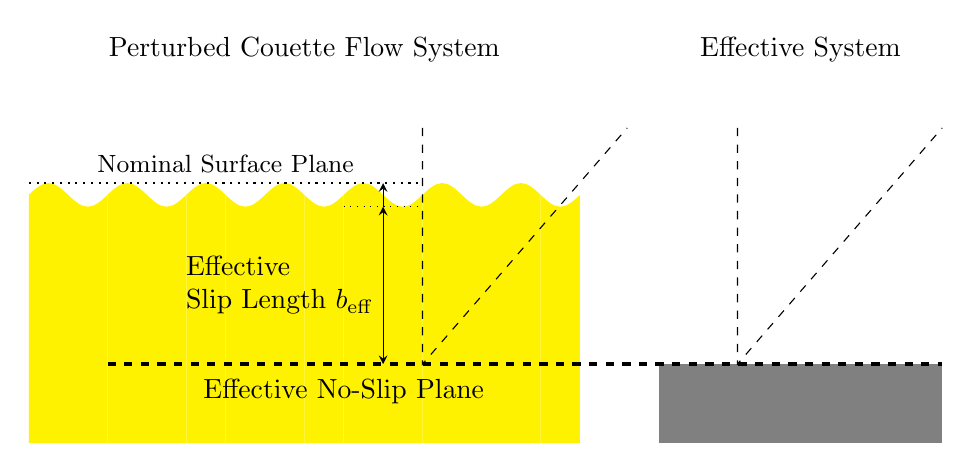
\begin{tikzpicture}  [> = stealth]
\renewcommand{\baselinestretch}{1.00}

%\fill[color=yellow] (0,0) rectangle (7,-3);

\foreach \x in {0,...,6}
               {   \fill[color=yellow] (\x,-3) -- ++(0,3.15) sin ++(0.25,0.15)
                   cos ++(0.25,-0.15) |- ++(-0.5,-3.15);   }
\foreach \x in{0,...,6} 
              {   \fill[color=yellow] (\x+ 0.5,-3) -- ++(0,3.15) sin ++(0.25,-0.15)
                  cos ++(0.25,0.15) |- ++(-0.5,-3.15);    }


\draw[dotted] (4,0) -- ++(1,0);
\draw[thick, dotted] (0,0.3) -- node[above]{\small Nominal Surface Plane} ++(5,0);

\draw [<->] (4.5,0) -- node[left, align=left] {Effective\\Slip Length $b_{\mathrm{eff}}$} ++(0,-2);
\draw [->] (4.5,0) -- ++(0,0.3);

\draw[dashed] (5,1) -- ++(0,-3) -- ++(2.6,3);

\fill[color=gray] (8,-2) rectangle ++(3.6,-1);
\draw[dashed] (9,1) -- ++(0,-3) -- ++(2.6,3);

\draw[very thick, dashed] (1,-2) -- ++(10.6,0);
\node at (4,-2.35) {Effective No-Slip Plane};

\node at (3.5,2) {Perturbed Couette Flow System};
\node at (9.8,2) {Effective System};
\end{tikzpicture}
\caption{Effective no-slip plane with rough surface} \label{rougheffnoslip} 
\end{figure}

\clearpage

\section{Purpose of Thesis}

The purpose of this thesis is to present a theory with which to predict the effective slip length, given knowledge of the local slip length:

\begin{equation}
b_{\mathrm{eff}} = f(b(x,y))
\end{equation}

Furthermore, the theory can deal with a rough surface, where the rough surface is described by a height function $h(x,y)$:
%Second, to extend the theory, taking into account the rough surface.

\begin{equation}
\beff = f(b(x,y),h(x,y))
\end{equation}

We present a formula for $\beff$, in the idealized case where surface roughness is periodic, and the local slip length varies with the same period, in the limiting case where the local slip length is always large compared to the period of surface roughness.

The answer turns out to be that $\beff$ is the area-weighted \emph{harmonic} average of the local slip length, where the area in question is the area of contact between solid and liquid.


\begin{equation}
\beff = \left< \frac{\sqrt{1+h'^{2}}}{b}  \right > ^{-1}
\end{equation}

The core of this thesis is a rigorous derivation of this result.

\vspace*{1em}
We also confirm, using a completely different mathematical technique, the special case of a flat surface:
\begin{equation}
\beff = \left< \frac{1}{b}  \right > ^{-1}
\end{equation}
We further show that for a flat surface, in the opposite limiting case where the period is large compared to any local slip length, that $\beff$ is the area-weighted average of local slip lengths:
\begin{equation}
\beff = \left< b  \right >
\end{equation}


\section{Application of Thesis}

%The question of whether or not fluid slips at the solid boundary is fundamental to fluid mechanics, in the sense that a %solution to the Navier Stokes equations requires a boundary condition, and the no-slip boundary condition was accepted by %consensus only after lengthy controversy.

The question of whether or not fluid slips at the solid boundary is fundamental to fluid mechanics in the following sense: To solve the Navier Stokes equation, a boundary condition is needed, and the no-slip condition was accepted by consensus only after lengthy controversy.
However, in almost all practical applications, plumbing, drainage, ship building etc., it turns out that any slip will be too small to matter.  At the macro scale, the no-slip boundary condition is observed.

Only recently has the possibility of fluid slip become important, in the new fields of microfluidics and nanofluidics.  In these fields, researchers and engineers fabricate devices in which fluid flows through pipes with a width measured in microns, or even smaller.  In such channels, the high surface area to volume ratio works strongly against fluid flow.  If the no-slip condition could be relaxed, then flow rates could be increased significantly.

Hydrophobic channel walls give the possibility of a non-zero intrinsic slip length.  However, larger slip effects are attempted by creating surfaces that contain regions of \emph{air,} perhaps trapped in small pockets on the surface.  Then the fluid flows partly over an air-water interface, which is expected to have a large intrinsic slip length. Experiments show increased flow rates through channels with such walls \cite{OuPerotRothstein2004, HyvaluomaHarting2008}.

The question is then \emph{how much} would flow rates increase with these exotic surfaces.  This can be rephrased as `what is the effective slip length of the surface?'  This thesis offers a means of calculating the effective slip length for some cases.

\clearpage

\section{Structure of Thesis}

The core of this thesis is essentially the shortest possible physically and mathematically rigorous derivation of the harmonic mean formula for $\beff$.  The remainder of the thesis consists of an alternative derivation of a special case of the harmonic mean formula, a derivation of another formula for $\beff$ in the complementary regime, some numerical testing, and a brief look at some analogues of effective slip in other physical systems.

Chapter 2 `Does Slip Exist?' reviews the literature on slip, focussing at reasonable depth on the (few) papers that credibly demonstrate intrinsic slip on a clean, atomically flat surface.  It ultimately concludes that an intrinsic slip length of 10 - 20 nm has been seen on hydrophobic surfaces.

Chapter 3 `Mixed Slip Flow' looks at flow over surfaces that are rough, or have a varying intrinsic slip length.  The focus is on `superhydrophobic' surfaces and nanobubbles, and the importance of carefully locating the $z=0$ plane.

Chapter 4 `Effective Slip Length Expressions: Prior Work' is a literature review of previous results for an effective slip length.  Since the work in this thesis has been published as three papers \cite{HendyLund2007, LundHendy2008, Lund2012}, the work is easily placed in context with other peer-reviewed articles.

Chapter 5 `The Mathematical Model' sets up the formal mathematical framework, including the definition and explanation of the velocity gradient tensor, and the simplification to Stokes flow.

Chapter 6 `The Homogenized Effective Slip Length' is the core of the thesis: The technique for solving partial differential equations known as homogenization is explained in some detail, and then applied to the effective slip problem.  An expression for $\beff$ is derived for the regime where the period is much smaller than any local slip length.

Chapter 7 `Perturbative Effective Slip Lengths' uses the completely different technique of perturbation methods to derive $\beff$ for the special case of a flat surface.  Also derived is another expression for $\beff$ that applies in the contrasting regime where the period is much larger than slip lengths.

Chapter 8 `Numerics' shows that numerical simulations using finite element modelling are in excellent agreement with our expression for $\beff$.

Chapter 9 `Analogues of Effective Slip' takes a brief look at other physical problems that happen to be described by a very similar mathematical model to that analysed in Chapter 5, and therefore have a similar solution.  A problem in thermal insulation, and a problem in catalysis are given a brief treatment.

Chapter 10 `Conclusion' summarises and considers future extensions to the work.


\section{Publications from the Work of this Thesis}

%The work of the this thesis has been published as three papers, with the second subsuming the first.  The first was written by my supervisor Dr Shaun Hendy, describing the use of a perturbation method to derive effective slip lengths for a one-dimensional flat surface \cite{HendyLund2007}.  I then extended the perturbation method to derive effective slip lengths for 3-D flow over a two-dimensional flat surface.  This work generalised the earlier result, and I wrote a paper describing it in 2008 \cite{LundHendy2008}.  I then used the homogenization method to derive an effective slip length for rough surfaces.  I wrote a paper describing this in 2012 \cite{Lund2012}.


The work of this thesis has been published as three papers, with the second subsuming the first.  The first was written by my supervisor Dr Shaun Hendy, after he developed a perturbative method to derive effective slip lengths for a one-dimensional flat surface, with analytical assistance from myself \cite{HendyLund2007}.  I then extended the perturbation method to derive effective slip lengths for 3-D flow over a two-dimensional flat surface.  This work generalised the earlier result, and I wrote a paper describing it in 2008 \cite{LundHendy2008}, with supervision from Dr Hendy.  Dr Xingyou `Philip' Zhang then introduced us to the homogenization method, which has a standard solution to a certain class of problems -- like ours -- characterized by periodicity.  With assistance from Philip, I applied the homogenization method to our problem, deriving an effective slip length for rough surfaces.  I then organized testing of the result via molecular dynamics simulations performed by a fellow student, Keoni Mahelona.  I wrote a paper describing this work in 2012 \cite{Lund2012}, with guidance from Dr Hendy and Dr Zhang.

\iftoggle{compilealone}
    {
    \bibliography{Lund_Thesis.bib}
    \bibliographystyle{plain}
    }

\end{document}
